% ------------------------------------------------
% Page start
% ------------------------------------------------
\chapter{Related Work}
\label{chapter:related-work}

\baselineskip=26pt
\thispagestyle{empty}
% ------------------------------------------------

% Query Language section
\subsection{Query Language}

There are many non-relational database can use the SQL-like query language to query the database, such as Apache Hive of Hadoop, Cassandra Query Language (CQL), N1QL of Couchbase, ArangoDB Query Language (AQL), Hypertable Query Language (HQL), Cypher in Neo4j, etc.\\

Alought they may useful to its own database, but all of them have a basic common problem --- total un-compatible with standard SQL. This problem is the main reason that causing a huge gap between the relational and non-relational database, which makes many application can't easy swap the database to seek for the benefit of distributed database.

% CQEngine section
\minisec{- CQEngine \cite{web:cqengine:official} -}
\medskip
CQEngine (Collection Query Engine) is a Non-relational database indexing and query engine, for retrieving objects matching SQL-like queries from Java collections, with ultra-low latency. 它提供多種indexing的功能, 有Hash, Unique, Compound, Navigable, RadixTree, ReversedRadixTree, InvertedRadixTree, SuffixTree, StandingQuery, Fallback.

\begin{figure}[h]
\centering
%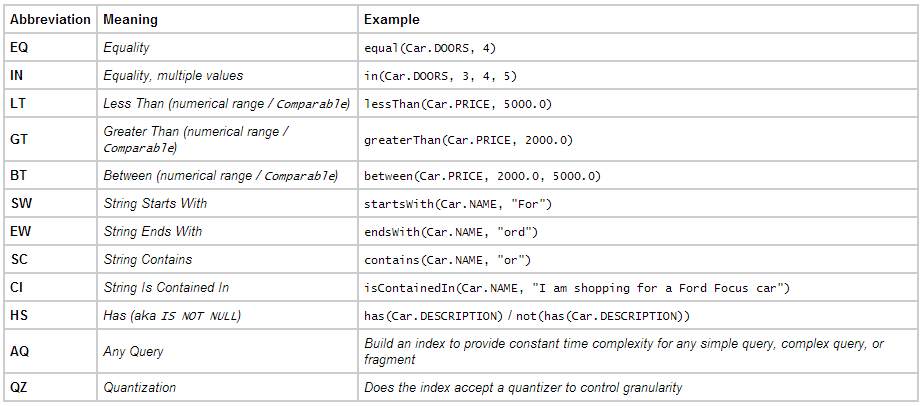
\includegraphics[scale=0.65]{./related-work/pic/CQEngine/CQEngine_index_1.png}
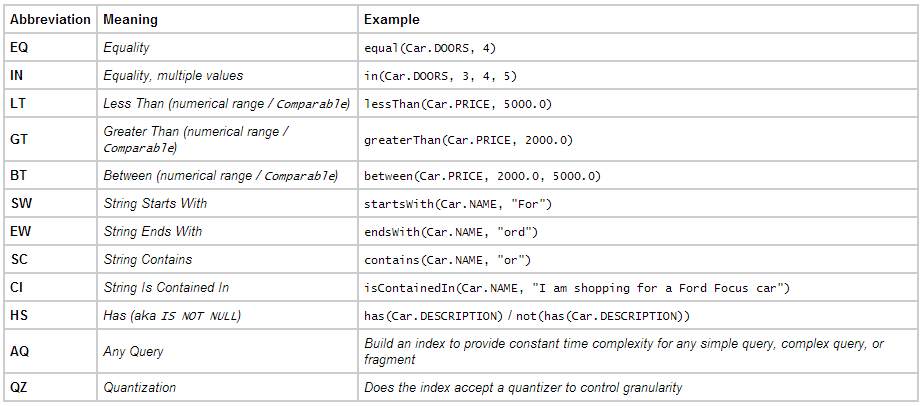
\includegraphics[width=0.8\textwidth]{./related-work/pic/CQEngine/CQEngine_index_1.png}
\caption{Legend for the feature matrix.}
\label{fig:related-work:legend_feature_matrix}
\end{figure}

\begin{figure}[h]
\centering
%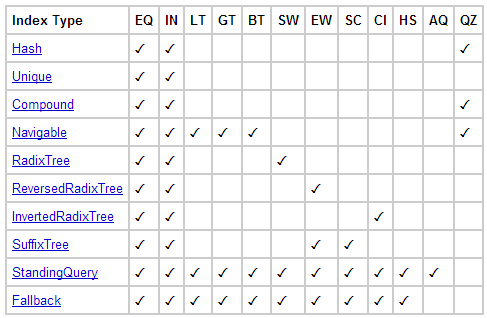
\includegraphics[scale=0.8]{./related-work/pic/CQEngine/CQEngine_index_2.png}
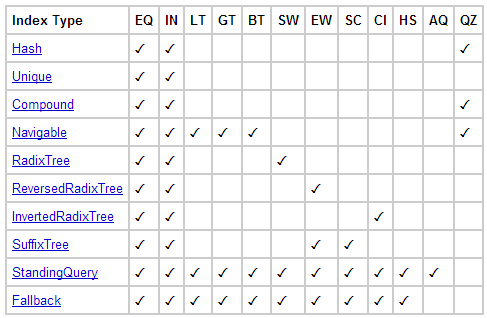
\includegraphics[width=0.8\textwidth]{./related-work/pic/CQEngine/CQEngine_index_2.png}
\caption{Index Feature Matrix.}
\label{fig:related-work:index_feature_matrix}
\end{figure}

User自己必須要定義自己的data是使用哪一定indexing的方式, 每一種indexing都只能做某一些特定的功能, 所以要先理解它們各自的特性.\\

雖然CQEngine是以indexing的想法來想提供key-value的application, 但它的使用方式卻不像現在的一些key-value的使用方式, 所以使用起來比較不friendly. From figure \ref{fig:related-work:example_useage}, we can see the simple of using CQEngine that the user need to define all the metadata.

\begin{figure}[h]
\centering
%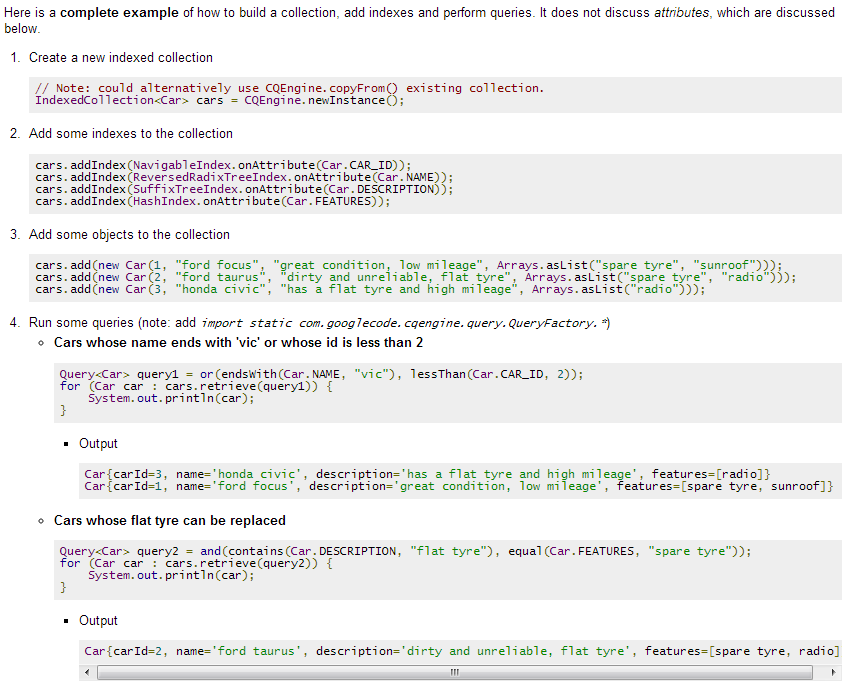
\includegraphics[scale=0.65]{./related-work/pic/CQEngine/CQEngine_index_3.png}
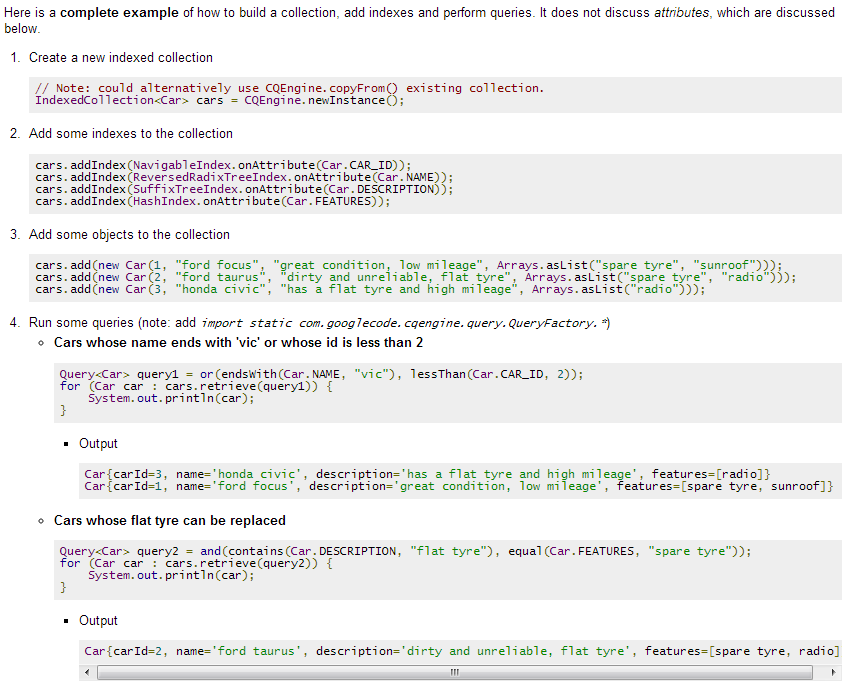
\includegraphics[width=0.9\textwidth]{./related-work/pic/CQEngine/CQEngine_index_3.png}
\caption{A complete example that how use the CQEngine.}
\label{fig:related-work:example_useage}
\end{figure}

CQEngine在想法上的確非常不錯, 但是CQEngine只有詳細說明query和indexing的效果和用法, 並沒有提及如何把data I/O到disk上, 所以可以假設它是in-memory database.

\clearpage

% Cassandra Query Language (CQL) section
\minisec{- Cassandra Query Language (CQL) \cite{web:cassandra:cql-tutorial} -}
\medskip
Apache Cassandra created by Facebook, Cassandra is a non-relational database distributed data store easily able to handle large amounts of writes and reads, a quality that has won favor with both high volume Internet services as well as with those firms executing big data-styled analysis.\\

\clearpage

% ArangoDB Query Language (AQL) section
\minisec{- ArangoDB Query Language (AQL) \cite{web:arangodb:aql-tutorial} -}
\medskip
AQL is a declarative query language similar to SQL and offers both simple and complex, nested queries. It can be used to retrieve data that is stored in ArangoDB.\\

\clearpage

% Storage engine section
\subsection{Storage engine}

So some research are maintain in relational database and do some improvement. Like \cite{paper:nodb,paper:spreadsheet-engine} are proposing swap the database engine to just use direct access the spreadsheet file (like CSV), which is very useful to some application and it can gain the benefit of distributed by using VFS (Virtual File System) mounting in Linux. This kind of design is suitable for common text and number data only, but not workable with the binary data like photos.

% NoDB section
\minisec{- NoDB \cite{paper:nodb} -}
\medskip
The authors in NoDB提出一個不用寫data到database, 就能以database的方式去query data的架構. 之後修改PostgreSQL來當成範例以證明NoDB是可以用在現在的database架構上, 在可用性和效率上得到好處.\\

他們提出了NoDB這個原因是去處理現在database技術中query反應的所需時間, 所以使用NoDB架構來減低讀取raw data的時間.\\

由於NoDB是設計成不用把data寫到database中, 所以它們的raw data是使用CSV files來當成data format, 之後database的任何行為都是在I/O CSV files. 而且data的indexing是使用dynamic allocation, 只有在處理query時才會產生出來, 而不是一直存在的, 所以不會需要有另外的indexing data在disk中.\\

這篇paper的確提出了一個新的做法去處理了一個到現在某些relational database系統中存在了40年的很基本的問題, 就是把所有data集中在一個地方. 問題就會出現在於如果要搬動database的話, 就要一整個database移動, 但如果database很大的話, this cost a huge of time. 但如果是多個CSV files, 在搬動時會十分方便, 而且可以控制mountpoint的方式去擴充database的空間, 這種擴充性也正是non-relational database在追求的其中一點.\\

而且因為data是CSV format, 但是不是任何data都是可以以CSV來處理, 例如non-structure和binary data, 這是data可能含有CSV用來分隔用的”comma”, 這會影響到讀取data的長度跟位置, 但是這篇paper中沒有討論相關的問題.

\clearpage

% Similar database section
\subsection{Similar database}

% Google F1 section
\minisec{- Google F1 \cite{paper:google-f1} -}
\medskip
To the best of our knowledge, Google F1 is the only one that can handle both kind of query (NoSQL and SQL) with fully functional in the current days.\\

Start from the Megastore (In chapter 3.2 of \cite{paper:google-megastore}), then up to the Spanner (At the introduction and chaper 2.3 of \cite{paper:google-spanner-1}) and the current F1 (Chapter 7 to 8 in \cite{paper:google-f1} or \cite{paper:google-f1-ad-business}). There is always mentioned about the SQL in the data model with the Protocol Buffer \cite{web:google:protocol-buffers}, this prove that even the database can be distrusted but still need a fully functional relational query interface to query the data which can't easy retrieve in a nomral \textit{get()} operation of non-relational database.\\

Google F1 is one of the database that can handle both kind of query (NoSQL and SQL) with fully functional in the current days. Start from the Megastore \cite{paper:google-megastore}, then up to the Spanner \cite{paper:google-spanner-1} and the current F1 \cite{paper:google-f1,paper:google-f1-ad-business} were always mentioned about the SQL in their data model.

% Conclusion section
\subsection{Conclusion}

This prove that even the database can be distrusted but still need a fully functional relational query interface to query the data which can't easy retrieve in a single \textit{get()} operation of non-relational database.

\clearpage

% ------------------------------------------------
% End of page
% ------------------------------------------------
